\documentclass[12pt]{article}

\usepackage[margin=1in]{geometry}
\usepackage{textcomp}
\usepackage{parskip}
\usepackage{amsmath}
\usepackage{authblk}
\usepackage[backend=bibtex, style=alphabetic, sorting=ynt]{biblatex}
\usepackage{graphicx}
\usepackage{wrapfig}
\usepackage{float}
\usepackage{caption}
\usepackage{setspace}
\usepackage{fancyhdr}
\usepackage{lastpage}
\usepackage{titlesec}
\usepackage{enumitem}
\usepackage{subfig}

\pagestyle{fancy}
\renewcommand{\headrulewidth}{0pt}
\renewcommand{\footrulewidth}{0pt}
\fancyhf{}
\lfoot{\scriptsize January 2019}
\cfoot{\scriptsize Brendon Matusch---Improving Particle Classification in WIMP Experiments}
\rfoot{\scriptsize Page~\thepage~of~\pageref{LastPage}}

\setlist[enumerate]{noitemsep, nolistsep}
\setlist[itemize]{noitemsep, nolistsep}

\graphicspath{{./images/}}

\addbibresource{paper.bib}

\titlespacing{\section}{0pt}{0pt}{0pt}
\titlespacing{\subsection}{0pt}{0pt}{0pt}
\titlespacing{\subsubsection}{0pt}{0pt}{0pt}

\doublespacing

\begin{document}

\begin{center}
    \begin{LARGE}
        Improving Particle Classification in WIMP Dark Matter Detection Experiments Using Neural Networks
    \end{LARGE}

    Brendon Matusch
\end{center}

\section{Introduction}

In all experiments for detection of Weakly Interacting Massive Particle (WIMP) dark matter, it is essential to develop a function that can distinguish events caused by WIMP candidates from those caused by background radiation. Manually developing such a classifier is challenging, time-consuming, and necessitates detailed physical modeling.

\begin{wrapfigure}{r}{0.4\textwidth}
    \centering
    \fbox{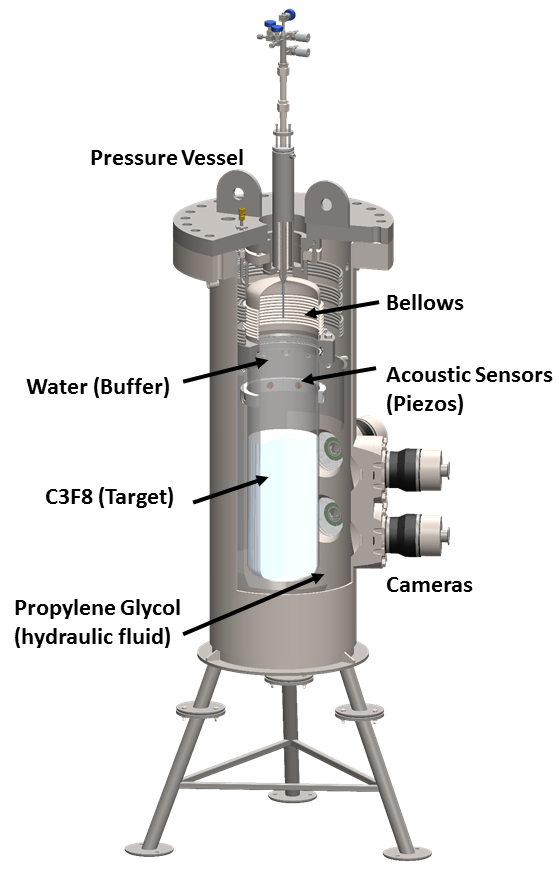
\includegraphics[width=0.38\textwidth]{pico_cad_cropped}}
    \caption{CAD rendering of the PICO-60 detector as configured for its operation with C$_3$F$_8$.}
\end{wrapfigure}

Machine learning (ML) has the potential to automate this and accelerate experimentation, in addition to detecting patterns that humans cannot. However, impure calibration data hinders training of models, and unusual detector topologies make data challenging to process.

Concretely, I worked with two dark matter experiments: the PICO-60 bubble chamber \cite{pico}, and the DEAP-3600 liquid argon scintillator \cite{deap}. In both experiments, alpha particles comprise a problematic class of background radiation. In PICO-60, WIMP-like neutron calibration events are used as training data; however, alpha particles mixed into this calibration data pose a challenge to effective training. In DEAP-3600, the detector format, containing 255 spherically arranged photomultiplier tubes (PMTs), making data processing challenging.

\begin{wrapfigure}{r}{0.4\textwidth}
    \centering
    \fbox{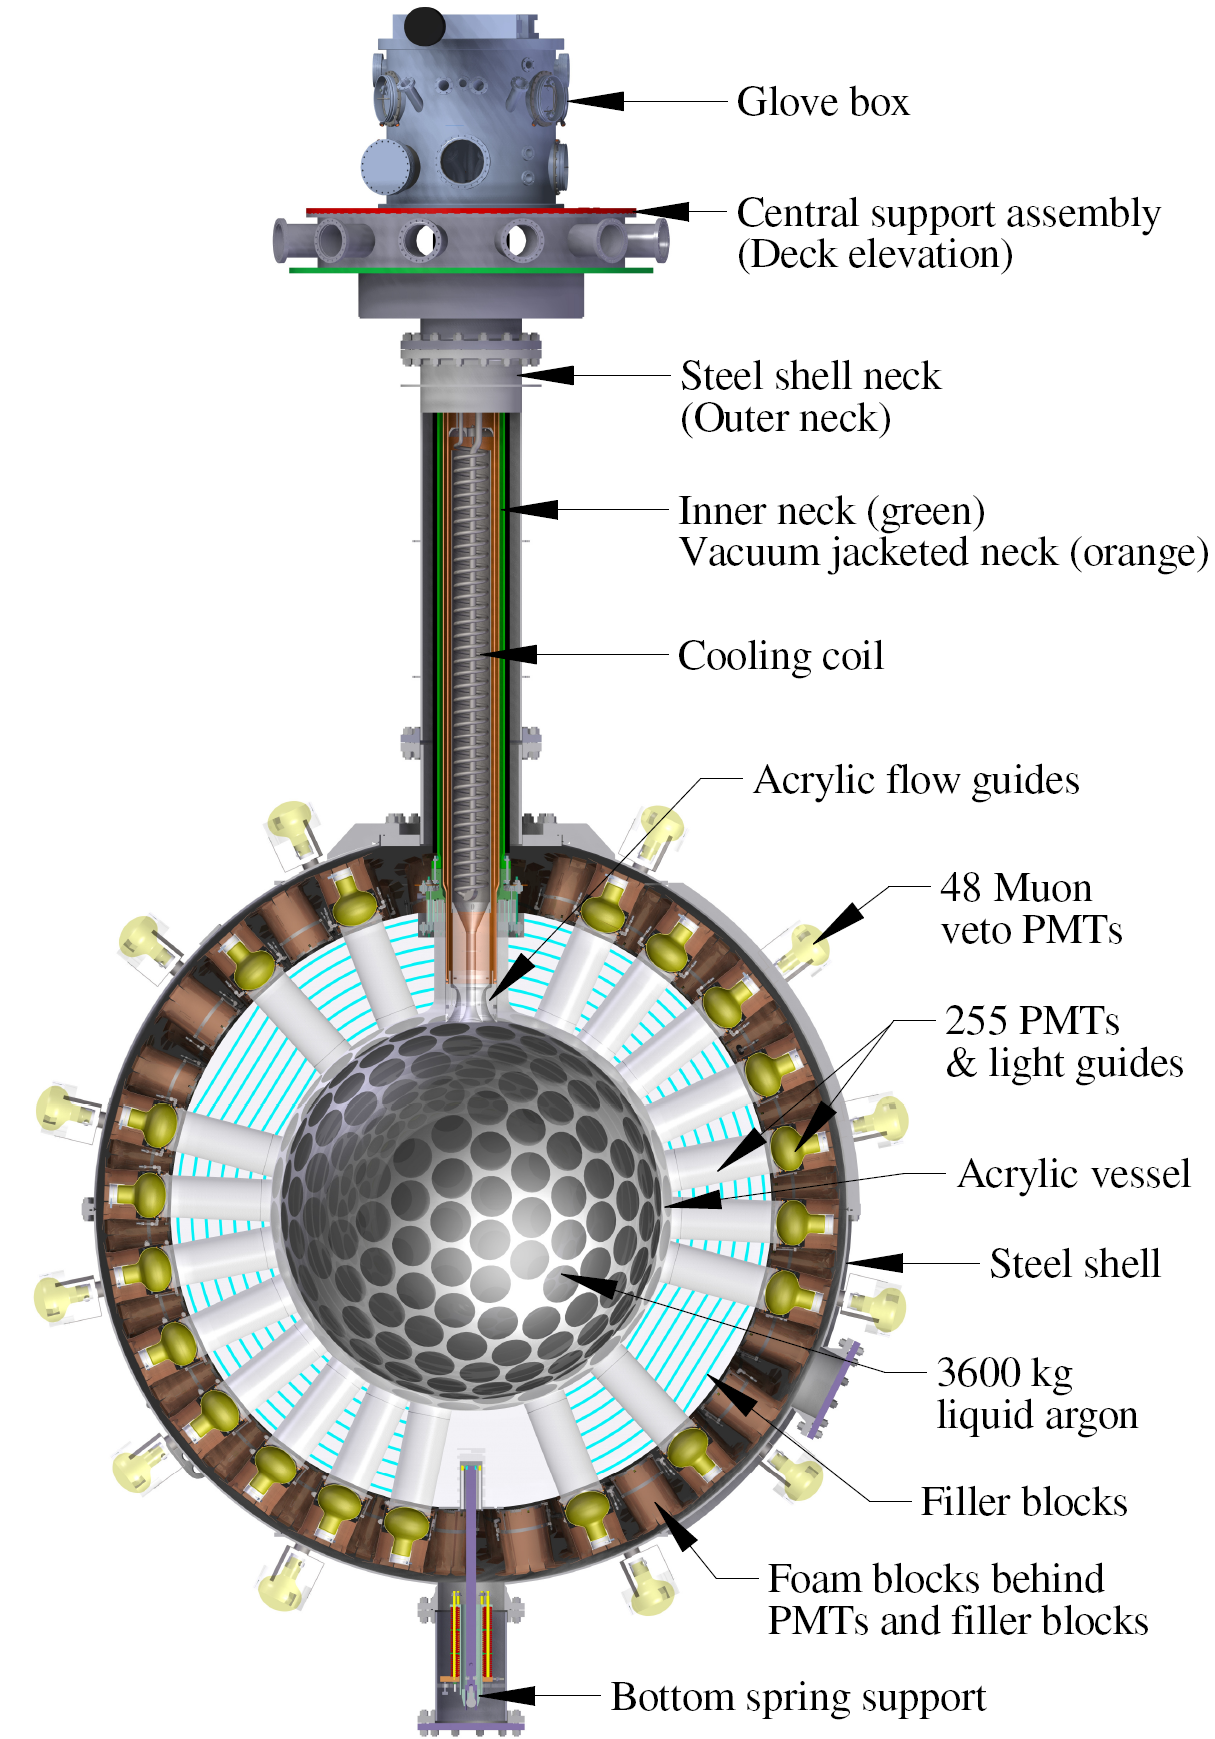
\includegraphics[width=0.38\textwidth]{deap_cad}}
    \caption{CAD rendering of the DEAP-3600 liquid argon scintillator.}
\end{wrapfigure}

In both experiments, conventional classifiers are typically used. In PICO-60, it is known to be nearly optimal; however, ML was additionally used (for its automation benefits), reaching a mean of 80.2\% accuracy. In DEAP-3600, in a simulated environment, the conventional classifier removes 99.6\% of alpha background radiation, while also (undesirably) removing 91\% of simulated WIMP events.

The objective of my study was to develop novel machine learning algorithms that perform better at this task than previous methods, in the PICO-60 and DEAP-3600 dark matter experiments, and I succeeded at this task. I have lead-authored an academic paper \cite{me} on my PICO-60 research, which the PICO collaboration has reviewed and approved.

\section{Procedure}

\subsection{PICO-60}

For PICO-60, I developed and compared two sets of classification algorithms:

\begin{enumerate}
    \item I experimented with conventional supervised learning (where a model is trained on a set of inputs with expected outputs). I explored the following data formats to learn which was the best-performing solution:
    \begin{itemize}
        \item An 8-band Fourier transform. I applied a dense neural network with dropout and L2 regularization (which allowed for less overfitting to impure data).
        \item A higher-resolution Fourier transform of the audio (all 50,001 data points). I once again applied a dense neural network.
        \item A raw audio waveform with a very deep 1D convolutional neural network (CNN) inspired by Dai et al \cite{verydeepconvnets}. I hoped to learn whether data preprocessing was required for good performance.
        \item Images captured by cameras in the detector. I trained a 2D CNN on these, to learn whether they contain any relevant information.
    \end{itemize}
    \begin{figure}[ht]
        \centering
        \subfloat{\fbox{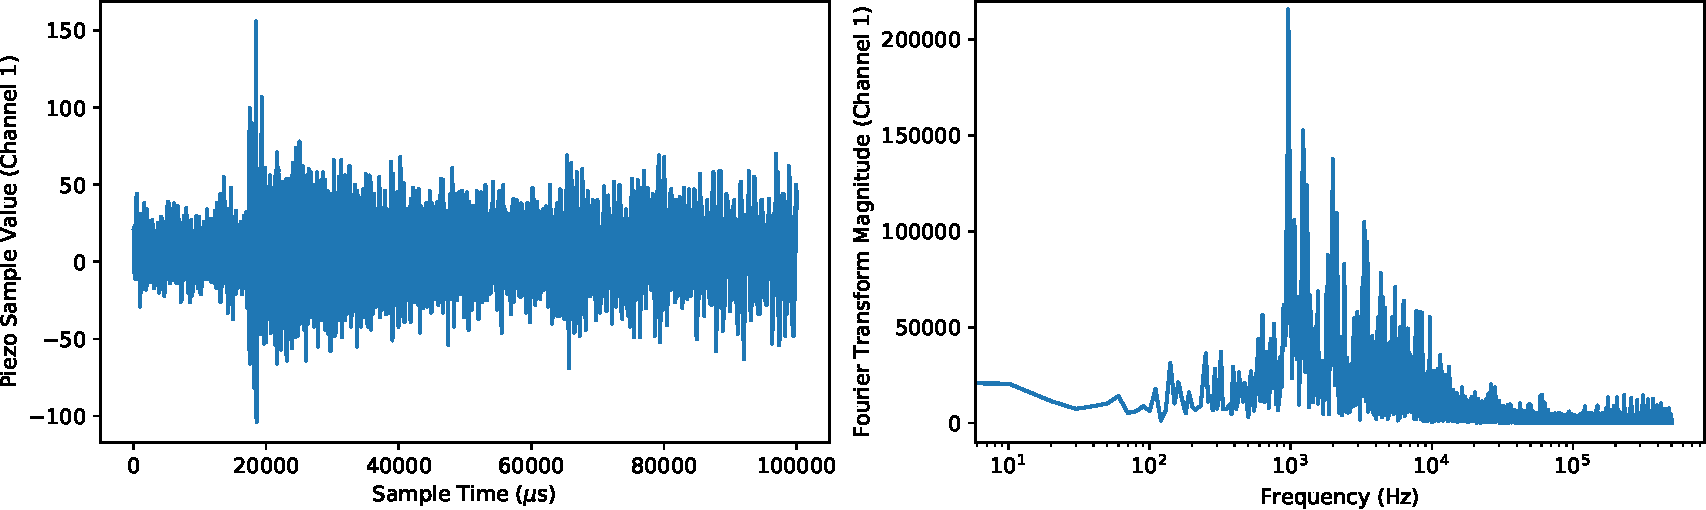
\includegraphics[width=0.9\textwidth]{audio_cropped}}}
        \qquad
        \subfloat{\fbox{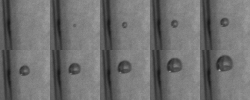
\includegraphics[width=0.45\textwidth]{image_grid}}}
        \caption{Examples of the audio waveform and Fourier transform (above) and the images captured by cameras (below).}
    \end{figure}
    \item The impurity in the training data was alleviated with regularization but not entirely solved. For a more optimal solution, I developed two entirely new semi-supervised learning algorithms. The particle labels (WIMP-like nuclear recoils, or alpha events) were removed from a large portion of the data, and my algorithms learned more accurate labels for this data.
    \begin{itemize}
        \item Iterative Cluster Nucleation is inspired by unsupervised "clustering" algorithms. First, a neural network is trained on a labeled set. After some time, it runs predictions on the unlabeled set. Those unlabeled examples with the most confident predictions (close to 0 or 1) are added to their corresponding cluster in the labeled set; these synthesized labels are more accurate than the original labels.
        \item Gravitational Differentiation is a more analog redesign. Using an original piecewise exponential function for calculating final-layer derivatives, called GravDiff, unlabeled examples are caused to "gravitate" toward more accurate predictions based on the confidence of the neural network's predictions.
    \end{itemize}
\end{enumerate}

\subsection{DEAP-3600}

In DEAP-3600, the key challenge is the aforementioned unusual detector format: a sphere tiled with a hexagonal lattice of PMTs. While it is fundamentally an image, conventional CNNs are intended only for flat rectangular images. I attempted to solve the problem in three different ways:

\begin{enumerate}
    \item I tried simply inputting photon counts from each PMT into a multi-layer perceptron, which has no awareness of spatial arrangement.
    \item The spherical image challenge is much like that cartographers face when making a map of the spherical Earth. I developed and applied a Mercator-inspired cylindrical projection to the spherical data, and used a 2D CNN.
    \item I developed an entirely new type of CNN, called a topological CNN. Rather than a 2D image of square pixels, kernels convolve over an arbitrary topology in any number of dimensions (in this case, a hexagonal lattice on the surface of a sphere).
\end{enumerate}

\begin{figure}[ht]
    \centering
    \subfloat{\fbox{
\includegraphics[width=0.45\textwidth]{map_projection}}}
    \qquad
    \subfloat{\fbox{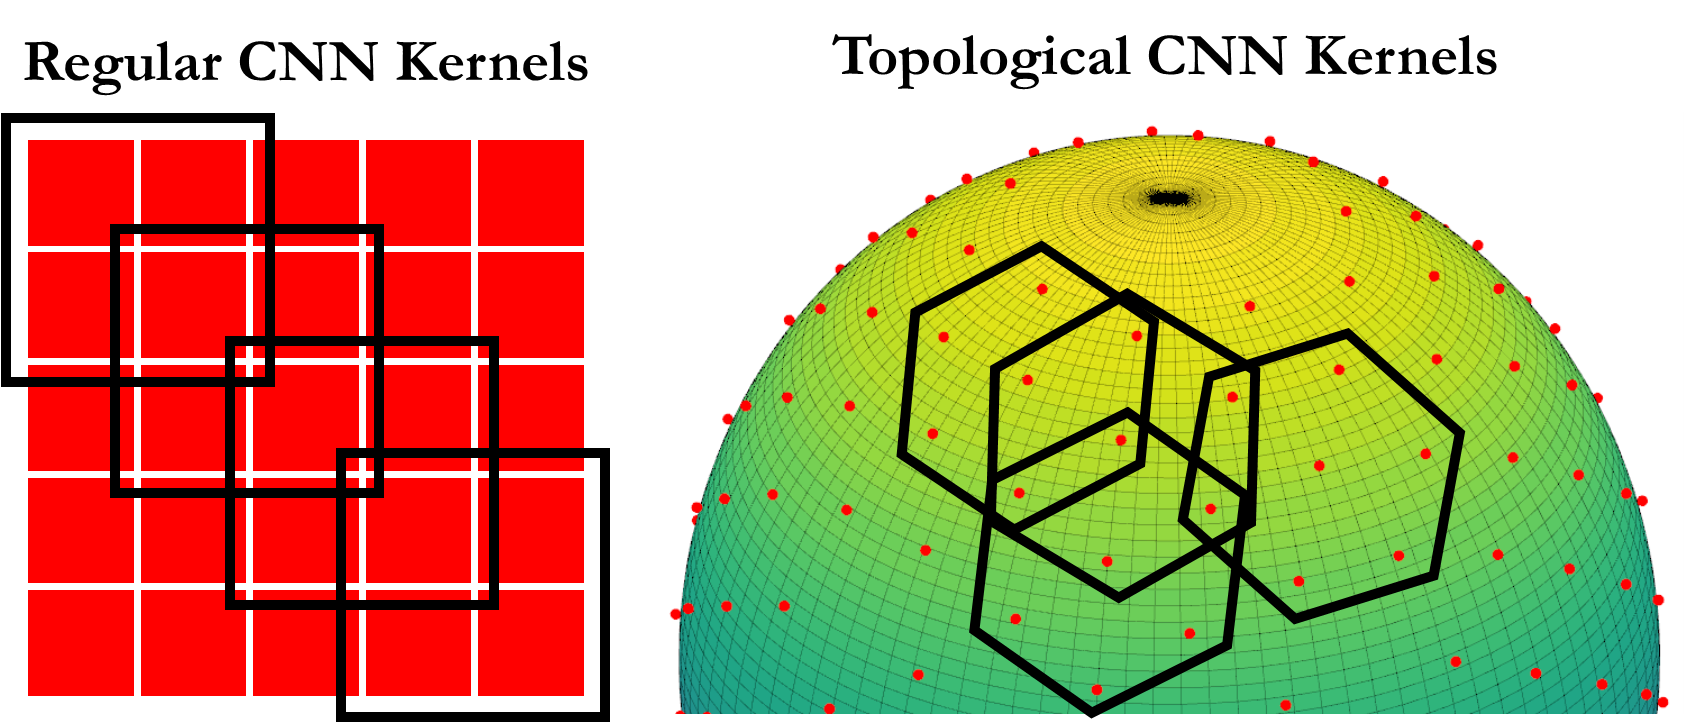
\includegraphics[width=0.45\textwidth]{topological}}}
    \caption{Diagrams of the map projection (left) and topological CNN (right) systems.}
\end{figure}

\subsection{Implementation}

ML algorithms developed in this study incorporated the Adam \cite{adam} and stochastic gradient descent \cite{sgd} optimizers, and applied dropout \cite{dropout} and L2 regularization.

All programming for this study was done in Python 3. Keras \cite{keras}, running on a TensorFlow \cite{tensorflow} backend, was used for all machine learning tasks. NumPy \cite{numpy} and SciPy \cite{scipy} were used for linear algebra and signal processing. ROOT \cite{root}, scikit-image \cite{scikit-image}, and scikit-learn \cite{scikit-learn} were used for data loading and storage. Matplotlib \cite{matplotlib} was used for data visualization.

\section{Results}

\subsection{Statistical Practices}

All performance statistics refer to a test set where specified, and a validation set elsewhere. Models were trained on a training set, and a separate randomly selected validation set was used to select the best-performing technique and corresponding hyperparameters (with a grid search). A test set was used to verify the performance of the model ultimately chosen.

\subsection{PICO-60}

\begin{itemize}
    \item The dense neural network, with banded Fourier transform input data, increased accuracy to 97.3\% on validation data, up from a previous best of 80.3\% with ML.
    \item The full resolution Fourier transform unexpectedly worsened accuracy to 92.2\%.
    \item The raw waveform with a 1D very deep CNN reached 94.5\% accuracy.
    \item Iterative cluster nucleation, using the dense network and banded input data, improved validation accuracy to 99.1\%.
    \item Gravitational differentiation was even more accurate, at 99.7\%.
    \item The best gravitational differentiation configuration was not as accurate on final test data as on validation data, but was much better than supervised learning, at 98.3\%.
\end{itemize}

\subsection{DEAP-3600}

The three architectures I tested for neck alpha identification in DEAP-3600 were evaluated based on their ability to reduce the rate of false positives (potential WIMP candidates misidentified as neck alphas) compared to the previous 91\% result from conventional methods. Only models with the same (or lower) 0.4\% false negative rate were considered.

\begin{itemize}
    \item The dense neural network always produced 100\% false positives.
    \item The topological CNN produced a false positive rate of 92.6\% (also worse than 91.0\%).
    \item The cylindrical projection method with a 2D CNN improved the false positive rate from 91.0\% to 75.7\% (a 63.0\% reduction)!
\end{itemize}

\section{Conclusion}

These results confirm that I achieved my goal. Indeed, semi-supervised learning for PICO-60 performed better than both the previous best result with machine learning, and my own supervised learning work. This significantly improves the accuracy that can be obtained quickly and without any manual optimization, allowing the team working on the experiment to iterate more quickly without the overhead of developing a conventional classifier.

The reduction in the false positive rate for DEAP-3600 provides evidence that machine learning is capable of improving the efficiency of this experiment. This may reduce the operation time required to collect sufficient data pointing towards the existence or non-existence of WIMP dark matter.

The classifiers developed during this study demonstrate great promise for machine learning in dark matter detection. Fundamentally, the problems I have solved with respect to PICO-60 and DEAP-3600 are not specific to these two experiments; they are common across many others. Thus, my algorithms are applicable in the broader field of dark matter detection.

\singlespacing
\printbibliography

\end{document}